% !TeX encoding = UTF-8
% !TeX program = xelatex
% !TeX spellcheck = en_US

\documentclass{cjc}

\usepackage{booktabs}
\usepackage{algorithm}
\usepackage{algorithmic}
\usepackage{siunitx}

\classsetup{
  % 配置里面不要出现空行
  title        = {GPU异构系统非对称内存访问现象的研究综述},
  title*       = {Title},
  authors      = {
    author1 = {
      name         = {作者名},
      name*        = {NAME Name-Name},
      affiliations = {aff1},
      biography    = {性别,xxxx年生,学位(或目前学历),职称,是/否计算机学会(CCF)会员(提供会员号),主要研究领域为*****、****.},
      % 英文作者介绍内容包括:出生年, 学位(或目前学历), 职称, 主要研究领域(与中文作者介绍中的研究方向一致).
      biography*   = {Ph.D., asociate profesor. His/her research interests include ***, ***, and ***.},
      email        = {**************},
      phone-number = {……},  % 第1作者手机号码(投稿时必须提供,以便紧急联系,发表时会删除)
    },
    author2 = {
      name         = {作者名},
      name*        = {NAME Name},
      affiliations = {aff2, aff3},
      biography    = {性别,xxxx年生,学位(或目前学历),职称,是/否计算机学会(CCF)会员(提供会员号),主要研究领域为*****、****.},
      biography*   = {英文作者介绍内容包括:出生年, 学位(或目前学历), 职称, 主要研究领域(与中文作者介绍中的研究方向一致).},
      email        = {**************},
    },
    author3 = {
      name         = {作者},
      name*        = {NAME Name-Name},
      affiliations = {aff3},
      biography    = {性别,xxxx年生,学位(或目前学历),职称,是/否计算机学会(CCF)会员(提供会员号),主要研究领域为*****、****.},
      biography*   = {英文作者介绍内容包括:出生年, 学位(或目前学历), 职称, 主要研究领域(与中文作者介绍中的研究方向一致).},
      email        = {**************},
      % 通讯作者
      corresponding = true,
    },
  },
  % 论文定稿后,作者署名、单位无特殊情况不能变更。若变更,须提交签章申请,
  % 国家名为中国可以不写,省会城市不写省的名称,其他国家必须写国家名。
  affiliations = {
    aff1 = {
      name  = {单位全名\ 部门(系)全名, 市(或直辖市) 国家名\ 邮政编码},
      name* = {Department of ****, University, City ZipCode, Country},
    },
    aff2 = {
      name  = {单位全名\ 部门(系)全名, 市(或直辖市) 国家名\ 邮政编码},
      name* = {Department of ****, University, City ZipCode},
    },
    aff3 = {
      name  = {单位全名\ 部门(系)全名, 市(或直辖市) 国家名\ 邮政编码},
      name* = {Department of ****, University, City ZipCode, Country},
    },
  },
  abstract     = {
    中文摘要内容置于此处(英文摘要中要有这些内容),字体为小5号宋体。
    摘要贡献部分,要有数据支持,不要出现“...大大提高”、“...显著改善”等描述,
    正确的描述是“比…提高 X\%”、 “在…上改善 X\%”。
  },
  abstract*    = {Abstract (500英文单词,内容包含中文摘要的内容). },
  % 中文关键字与英文关键字对应且一致,应有5-7个关键词,不要用英文缩写
  keywords     = {关键词, 关键词, 关键词, 关键词},
  keywords*    = {key word, key word, key word, key word},
  grants       = {
    本课题得到……基金中文完整名称(No.项目号)、
    ……基金中文完整名称(No.项目号)、
    ……基金中文完整名称(No.项目号)资助.
  },
  % clc           = {TP393},
  % doi           = {10.11897/SP.J.1016.2020.00001},  % 投稿时不提供DOI号
  % received-date = {2019-08-10},  % 收稿日期
  % revised-date  = {2019-10-19},  % 最终修改稿收到日期,投稿时不填写此项
  % publish-date  = {2020-03-16},  % 出版日期
  % page          = 512,
}

\newcommand\dif{\mathop{}\!\mathrm{d}}

% hyperref 总是在导言区的最后加载
\usepackage{hyperref}



\begin{document}

\maketitle


\section{引言}

近年来,信息技术的迅猛发展和应用普及所带来的数据爆炸性增长,通用计算领域图形处理器GPGPU(General-Purpose Computing Graphics Processing Unit)由于其强大的并行计算能力、高吞吐率以及高性价比,已经成为高性能计算领域的主流加速器。基于GPGPU的计算加速成为了高性能计算、机器学习和数据分析应用的主要工具。这些领域的进一步发展依赖于GPU性能的进一步拓展,直到近几年,GPU一直通过晶体管数量的增加来增加SM的数量从而来拓展性能。

但是,随着晶体管缩放速度的放缓,晶体管密度增长速度放缓,同时随着GPU接近最大芯片尺寸的限制,单GPU性能拓展速度进一步放缓。同时,伴随着数据量的爆炸性增长,很多应用程序已经能够完全占用单GPU上的计算资源,这需要GPU系统性能的进一步拓展来满足人们的需要。通过将多个单片GPU拓展为多GPU系统,通过系统集成来提升应用程序性能是一种有效的解决方案。目前系统正逐渐向CPU与多GPU互联的异构系统拓展。

但是多GPU异构系统带来了一系列问题。例如,跨GPU的工作分配不容易透明地完成,同时在工作分区、负载平衡和同步方面也面临着一系列挑战。此外,多GPU的性能很大程度依赖着多级系统的互联,沿着这些互联传递的同步信息和数据移动显著影响着多GPU系统的整体性能和功效。本文重点关注了多GPU系统中存在的非对称内存访问的现象,主要包括以下几个方面:(1)GPU内存架构,以此为基础所存在的三种非对称内存访问的问题;(2)CPU与GPU互联的带宽差距以及解决方案,主要是GPU初始化时的数据布局和线程调度;(3)GPU内部多级内存的非对称内存访问的解决方案,主要包括数据布局,线程调度和互联网络优化;(4)多GPU互联的非对称内存访问的解决方案,主要包括封装架构,数据布局以及线程调度等方法;(5)目前的发展特点以及未来的坊站方向。本文的第2节介绍GPU的内存架构,特别是他们之间的带宽差距;第3节介绍了几种非对称内存访问的解决方案;第4节介绍了目前的主要挑战和未来的发展方向。

\section{GPU异构系统的内存架构}

随着单GPU向着多GPU拓展,逐渐形成了CPU与GPU构成的异构系统,其中CPU可以与GPU进行数据传递,不同GPU之间也可以相互通信。而数据传递的带宽差距是导致非对称内存访问的主要原因。为了更好的对GPU异构系统的非对称内存访问进行研究,需要对GPU的内存架构进一步了解。在GPU异构系统中,存在三方面的主要通信,分配内存和线程时的CPU与GPU的通信,GPU内部数据的移动,以及GPU之间的数据传递。因此在这种系统中,存在三种可能导致非对称内存访问现象的行为。

(1)由于CPU和GPU的存储器是分离的,CPU端的内存被称为Host(主机)内存,GPU端的内存被称为Device(设备)内存。如果需要在GPU端进行计算,就需要把待处理的数据拷贝到device内存中,待数据处理完成后,还需要把计算结果拷贝到Host端做进一步的处理,比如存储到硬盘中或者打印到显示器上。在这种系统中,GPU以高带宽访问本地存储器,为了完成这一系列操作,需要CPU与GPU之间进行数据传递,但是CPU与GPU互联的带宽很低,这导致了这种情况下非对称内存访问的产生。

(2)在CPU分配完程序数据后,对于GPU而言,数据处在带宽相对较低的DRAM之中。对于GPU的每个计算内核来说,他们都有着属于自己的私有L1缓存,同时所有内核通过互连网络与L2缓存相连接。当数据在L1缓存中发生失效时,内存请求会被发送到L2缓存中,如果在L2缓存中也发生了失效,内存请求才会被发送到DRAM中。由于访问L1缓存的速度要远远超过访问L2级缓存和访问DRAM的速度,因此,如果数据在L1缓存中失效,就需要花费好几倍的事件去低级cache中进行查找,这导致了这种情况下非对称内存访问的产生。

(3)对于多GPU系统来说,由于程序和数据被分配到多个GPU的存储器中,GPU内部的数据被称为本地数据,而存放在其他GPU上的数据被称为远程数据。一般来说,访问本地数据的过程和单GPU内部访问流程一样,而访问远程数据则需要通过PCIe或者NVLink等发送到远程GPU来进行处理。多GPU系统中的通信主要通过两种主要的机制来进行实现:数据页迁移和远程直接内存访问。

数据页迁移,首先需要GPU1的计算单元产生内存请求,地址转换请求发送到IOMMU进行服务时,检测到GPU不存在该页面,触发页面错误由GPU驱动程序进行处理,GPU的驱动程序在接收到页面错误请求时,使数据所在的GPU2进行刷新,来保证数据一致性,刷新包括流水线刷新,cache写回以及TLB更新等,刷新之后,数据页迁移控制器将数据页从GPU2迁移到GPU1,并通知驱动程序页面迁移已经完成。然后驱动程序让GPU2开始继续执行,GPU1通过更新的地址转换来访问获得的数据。

远程直接内存访问,当GPU1的处理单元需要访问数据时,向L1缓存发送请求,在TLB的帮助下转换地址,由于数据不再本地GPU中,转换请求被发送到IOMMU之中,IOMMU会返回远程GPU物理地址,而不是触发页面错误,接收到远程GPU上的物理地址转换,L1缓存将内存请求重定向发送到远程GPU的L2缓存中获取数据。这种方式获得的数据不会被缓存。

目前多GPU互联的技术,NVLink只能提供300GB/S的带宽,与DRAM的1TB/S的带宽仍有着较大的差距,并且,论文《Tartan: evaluating modern GPU interconnect via a multi-GPU benchmark suite》表明,很难充分利用GPU互联的全部带宽,这导致了非对称内存访问的产生。

图带宽差距比对。

非对称内存访问现象在CPU已经出现过,在多核CPU系统上,很多都是通过软件内存分配和迁移策略,以及线程调度等技术来最小化非对称内存访问带来的性能损失。这些解决方案大多是反应式解决方案,运行时进行检测位置和拥塞情况来进行数据迁移,数据复制和线程调度等。而在GPU中,由于GPU运行的程序大多是并行程度较高的应用程序,数据迁移可能会导致频繁的刷新流水线,产生高额的开销;数据复制可能会增大内存的压力,导致缓存抖动等现象;GPU运行的大量线程也使得线程调度变的复杂。因此,如何能够有效地解决GPU异构系统的非对称内存访问是目前的主要问题之一。本文主要针对了GPU异构系统的非对称内存访问来研究解决方案。

\section{GPU异构系统的非对称内存访问}

\subsection{CPU与GPU互联}

将CPU与GPU结合的异构系统能够有效地提升系统整体性能,但是非对称内存访问会阻碍性能的进一步发展。为了减轻非对称内存访问的影响,更好的从系统中获益,需要充分考虑分配到不同设备上的工作负载和数据。如果盲目的进行分配,可能会造成分配到GPU上的数据不能被分配的线程充分的利用,从而造成因无效数据传输而带来的性能损失,从而导致系统整体性能下降。因此在CPU-GPU异构系统中,更需要合理的对数据和线程进行分配,同时寻求合理的减少数据通信损失的方法。

\begin{figure}[htb]
  \centering
  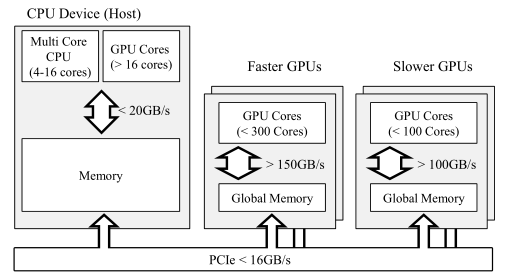
\includegraphics[width=\linewidth]{1.png}
  \caption{图片说明 *字体为小 5 号,图片应为黑白图,图中的子图要有子图说明*}
\end{figure}

\subsubsection{数据布局}

CPU和GPU上的异构计算传统上对每个设备使用固定的角色:GPU通过利用其大量内核来处理数据并行工作,而CPU处理非数据并行工作,如顺序代码或数据传输管理。再过去的方法中,通常通过程序员来进行数据分配,这容易出现错误,并且随着程序数据量扩大显得越发复杂。因此,需要一种动态的不需要干预的方式来对程序数据进行合理的分配。

由于使用GPU运行的主要是并行的应用程序,为了减少数据移动,数组上线界确认移动。

但是数组上下界准确率,提出了计算网格分解一维,同时充分考虑DRAM的共享。

扩展到多维,增加对内核外数据的考虑

同时,由于GPU发生页故障,需要PCIe向CPU相应,提出了远程数据的MSHR以及数据预取机制。

\subsubsection{互连网络}

拓扑结构,利用多GPU的通信模式和覆盖网络


\subsection{GPU内部}

在CPU进行数据分配之后,GPU的存储结构决定了大部分的数据会存放在带宽较低的DRAM中。对于GPU内部而言,虽然访存延迟可以通过切换线程来进行隐藏,但是对于大部分应用程序,尤其是存储密集型应用程序来说,访存的高额延迟无法被有效的隐藏,线程被阻塞,等待访存操作的完成,这也就是所说的存储墙的问题。为了解决速度不匹配的问题,通常需要减少访问低级cache的次数和降低访问的延迟。因此我们从数据,线程以及互联网络这三个方面进行考虑。

\subsubsection{数据布局}

\textbf{数据分配}

对于单GPU来说,由于L1 cache的容量有限,只能将程序所需要的部分重要数据放在L1 cache中。对于程序所需要的数据,需要对数据进行静态分配或者对数据进行动态迁移到使用数据的内核中。

首先GPU上运行的主要是并行程度高的应用程序,循环和数组,可以通过对程序进行预先分析,从而实现对数据的静态分配。介绍论文《Compiler Support for Selective Page Migration in NUMA Architectures》通过编辑器分析程序中的循环和数组变量。

但是静态分配无法分析GPU在运行过程中产生的信息,比如说数据迁移和计算放置等信息,这可能会产生一定的错误分配从而导致性能下降。过去曾经在CPU提出过的动态页面迁移,在GPU中很难取得很好的效果,在GPU中进行动态页面分析和迁移的成本可能非常高,并且GPU中进行页面动态迁移可能导致的页面锁,流水线刷新,提高开销。

\textbf{数据保护}

由于L1 cache的容量有限,对于已经进行页面分配存放到L1 cache中的数据来说,可能会由于未来访问的数据而被替换掉,这些数据如果在未来被使用,就需要重新到更低级cache中访问,从而导致性能下降。为了保护数据的局部性,从而保证数据复用,需要采取一定的策略来进行数据保护。

对于cache来说,为了预防抖动导致可能会复用的数据被刷新,因此需要采取合适的策略来保护具有空间和时间局部性的数据。

介绍论文《Access Pattern-Aware Cache Management for Improving DataUtilization in GPU》
缓存保护(得知复用的周期),缓存旁路等方法。

同时,传统的L1 cache是每个SM所私有的,但是实验证明,大多数内核所需要的数据可以从其他内核中找到。共享L1 cache。

\subsubsection{线程调度}

为了更好地对数据进行复用,除了对数据进行调度外,还可以通过对线程调度来实现。

指令链卸载到存在数据的GPU之中。PIM,介绍论文《2016 Scheduling Techniques for GPU Architectures with Processing-In-Memory Capabilities》

更好的利用cta间的局部性,从而复用L1 cache。介绍论文《2017 Locality-Aware CTA Clustering for Modern GPUs》

\subsubsection{互联网络}

对于L1 cache中发生失效的数据,必须通过互联网络发送到L2中进行访问。

虚拟通道,轮询使用

对于GPU内部来说,内核发出的内存请求的数据如果在L1中失效,会通过互联网络将内存请求发送到L2中。MC的分配,介绍论《Bandwidth-efficient On-chip Interconnect Designs for GPGPUs》


\subsection{GPU互联}

多GPU互联时的非对称内存访问现象相对于CPU-GPU以及GPU内部来说更为复杂,由于程序内核之间的依赖性,多GPU之间可能需要更为频繁的数据传递,同时虽然GPU内部访问DRAM的带宽相对较低,但通过PCIe等方式访问其他GPU的带宽与DRAM带宽相差一个数量级以上,这使得多GPU的非对称内存访问现象更加的复杂和显著。同时,由于多GPU的存储器相互分离,一份数据可能在多个GPU的存储器中含有拷贝,如何在保证数据一致性的基础上进行数据移动是多GPU面临的一个主要问题和挑战。为了更好的减轻多GPU的非对称内存访问的影响,在保证数据一致性的基础上,从软件和硬件两种角度充分的复用远程数据并降低访问远程数据的开销是目前主要的解决思路。

\subsubsection{数据布局}

\textbf{数据分配}

对于多GPU来说,页面一开始是通过CPU来进行分配的,为了减少多GPU之间通信。

首先数据分解

保证数据结构对齐

基于带宽的页面分配

在程序运行过程中,通过页面迁移,包括数据预取等
  
\textbf{数据保护}

多GPU之间共享数据,划分DRAM的cache,以及缓存旁路(确定那些数据是远程数据)等方法来提升性能。

\subsubsection{线程调度}

全局CTA调度,减少GPU之间的通信

\subsubsection{封装架构}

对于多GPU来说,未来的拓展方向主要有两个

将单GPU划分为多个module

将多个GPU通过交换机连接起来

通过API来自由选择GPM和多GPU互联

\section{挑战与展望}

随着工艺的进一步发展,目前的主要研究方向是多GPU互联的性能问题。

  (1)与理想情况仍有性能差距,多GPU互联性能超过线性相加的性能。

  (2)保持cache一致性问题

未来的发展方向

  (1)提出更合理的多GPU封装方法

  (2)更好地结合软硬件方法,提升性能

  (3)保持cache一致性的基础上降低通信开销


\end{document}
